% Semantic Assistants - http://www.semanticsoftware.info/semantic-assistants

% This file is part of the Semantic Assistants architecture.

% Copyright (C) 2009, 2010, 2011 Semantic Software Lab, http://www.semanticsoftware.info
% The Semantic Assistants architecture is free software: you can
% redistribute and/or modify it under the terms of the GNU Affero General
% Public License as published by the Free Software Foundation, either
% version 3 of the License, or (at your option) any later version.
   
% This program is distributed in the hope that it will be useful,
% but WITHOUT ANY WARRANTY; without even the implied warranty of
% MERCHANTABILITY or FITNESS FOR A PARTICULAR PURPOSE.  See the
% GNU Affero General Public License for more details.
 
% You should have received a copy of the GNU Affero General Public License
% along with this program.  If not, see <http://www.gnu.org/licenses/>.

\chapter{Developer Notes}
\label{chap:dev}
In this chapter, we provide additional information for developers. 
\begin{figure}[t]
  \centering
  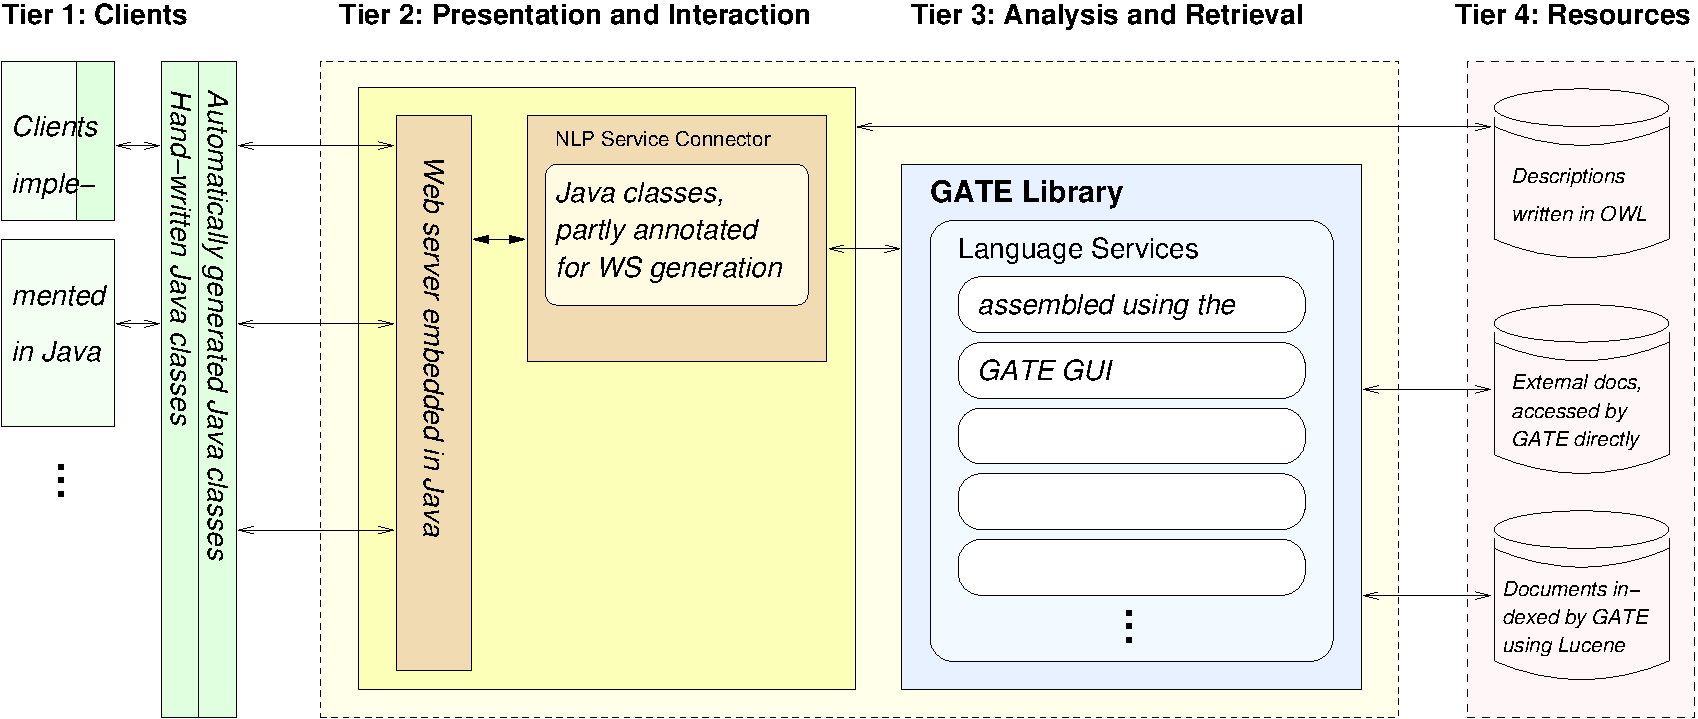
\includegraphics[width=\textwidth]{pictures/arch_impl}
  \caption{The architectural overview with implementation notes}
  \label{fig:arch_impl}
\end{figure}

\section{Project Description}
This section gives an overview of the directory structure and explains the modifications
required for every user to be able to proceed with the compilation.

\subsection{Top-Level Directory Structure}
The implementation of the architecture is located in
\url{SemanticAssistants/}. There are the following directories:
\begin{description}
\item[Clients:] contains all clients (OpenOffice, CommandLine, Eclipse)
\item[CSAL:] constain ths client-side abstraction layer code
\item[Doc:] contains this documentation
\item[Lib:] contains 3rd-party libraries
\item[Resources:] contains the upper ontologies, as well as the
  example OWL service descriptions and corresponding GATE pipelines
\item[Server:] contains the \sa server code
\end{description}
In addition, there are a number of files:
\begin{description}
\item[build.xml] used for executing code analysis tools
\item[LICENSE.txt] the APGL3 license for the \sa architecture
\item[LocalProperties.xml] optional customatizations, e.g., for local
  classpaths or overriding the default locations of the NLP services
\item[SemassistProperties.xml] properties file evaluated by ant when
  compiling or running the various parts of the \sa architecture
\end{description}

\paragraph{Generic Compilation Instructions:}
All parts of the \sa architecture (server, CSAL, clients) come with
ant build scripts that allow compilation from the command line
(usually \texttt{ant compile} or \texttt{ant run}).

\subsection{Server Directory Structure}
The following directories and files are found under the \emph{Server} directory.

\begin{enumerate}
\item \url{src}: Contains the java source code.
\item \url{gate-home}: Contains two gate user configuration files \emph{gate.xml} and \url{user-gate.xml}.
\item \url{logs}: It is used for server log files.
%\item \url{nbproject}: Contains configuration and properties files used by the NeatBeans IDE if the \emph{Server} is loaded through Netbeans.
%\item \url{.classpath}: ClassPath file for NetBeans.
%\item \url{.project}: Project Description file for NetBeans.
\item \url{Makefile}: Makefile that can be used to invoke Ant targets.
\item \url{build.xml}: Ant build file use to compile the project. Contains dependency information.
%\item \url{nb-build.xml}: Build file used by Netbeans.
\item \url{protege.properties}: Generated properties file, used by Protege.
\item \url{build}: Contains the binary java .class files.
\item \url{dist}: Contains a .jar file of the compiled server side.
%\item \url{nbdist}: Contains a .jar file of the compiled server. Generated when the server is compiled through Netbeans.
\end{enumerate}


\subsection{CSAL Directory Structure}
The following directories and files are found under the \emph{CSAL} directory.

\begin{enumerate}
\item \url{src}: Contains the java source code of the client side abstraction layer.
\item \url{dist}: Contains the output .jar file result of compilation of the CSAL.
%\item \url{nbproject}: Contains configuration and properties files used by the NeatBeans IDE if the \emph{CSAL} is loaded through Netbeans.
%\item \url{.classpath}: ClassPath file for NetBeans.
%\item \url{.project}: Project Description file for NetBeans.
\item \url{Makefile}: Makefile that can be used to invoke ant targets.
\item \url{build.xml}: Ant build file use to compile the project. Contains dependency information.
\item \url{bin}: Contains the binary java .class files.
%\item \url{nb-build.xml}: Buildfile used by Netbeans.
\end{enumerate}


\subsection{Clients Directory Structure}
The two sample clients we provide, \emph{CommandLine} and \emph{OpenOffice}, have the following directory structure.

\subsubsection{Command Line Client Directory Structure}
\begin{enumerate}
\item \url{src}: Contains the java source code of the Command Line Client.
%\item \url{nbproject}: Contains configuration and properties files used by the NeatBeans IDE if the \emph{Command Line Client} is loaded through Netbeans.
%\item \url{.classpath}: ClassPath file for NetBeans.
%\item \url{.project}: Project Description file for NetBeans.
\item \url{build.xml}: Ant build file use to compile the project.Contains dependency information.
\item \url{bin}: Contains the binary java .class files.
\item \url{runclient.sh}: Script helps with the class path setting and running the client.
\item \url{usableCommands}: Example of commands that can be invoked when running the runclient.sh script.
\end{enumerate}

\subsubsection{OpenOffice.org Writer Client Directory Structure}
\begin{enumerate}
\item \url{src}: Contains the java source code.
\item \url{dist}: Contains the \emph{Addons.xsu}, \emph{Protocolhandler.xsu} and \emph{ProtocolHandlerAddon\_ java.uno.jar} files.
\item \url{build.xml}: Ant build file use to complile the project.Contains dependency information.
\item \url{bin}: Contains the binary java .class files.
\item \url{SemassistOpenOfficePlugIn.oxt}: Contains the output file result of complilation and packaged in oxt plug-in format used by OpenOffice.
%\item \url{nbproject}: Contains configuration and properties files used by the NeatBeans IDE if the \emph{Command Line Client} is loaded through Netbeans.
%\item \url{nb-build.xml}: Buildfile used by Netbeans.
\end{enumerate}

\subsubsection{Eclipse Client Directory Structure}
\begin{enumerate}
%\item\url{icon}: This is where the SA icon images are stored.
\item \url{src}: This folder contains the Semantic Assistants plug-in source
code. The internal structure of this directory is further explained in section
\ref{subsec:eclipse.development}.
\item \url{lib}: This is where all the external plug-in dependencies are stored.
This folder contains the Client-Side Abstraction Layer JAR file used in the
project to communicate with the server.
\item \url{plugins}: This is where the Semantic Assistants plug-in JAR file will
be stored when successfully built.
\item \url{META-INF}: This is where the plug-in manifest file is stored. This
file is used by the Eclipse plug-in loader to identify the Semantic Assistants
plug-in.
\item \url{plugin.xml}: This file
contains general information of the plug-in like its dependencies, runtime
classpath and extension points in form of an XML file and is used to
introcude the plug-in to Eclipse plug-in loader. By using this file, developers
can test the plug-in inside an Eclipse runtime application.
\end{enumerate}


\section{Server and CSAL Compilation} 
\label{sec:inst-comp}
To compile and start the server and compile the CSAL, follow these
steps:

\begin{enumerate}
  \item cd to \emph{Server}

  \item \texttt{ant run}. The server is built and should come up, with
    some debug output on the console.

  \item with the server running, cd to \emph{CSAL}

    \begin{enumerate}
    \item \texttt{ant dist}. This builds the client-side abstraction
      layer (CSAL) that all (Java) clients should use to connect to
      the architecture (i.e., the server). Note that the server must
      be running for the client to be built, because the code
      generation step imports the server's WSDL definitions. In
      addition, the WSDL definitions are cached localy.
      % where exactly?
      
      \item \texttt{ant dist-offline} This builds the client-side
      abstraction layer (CSAL) with the cached WSDL definitions during
      a previous on-line compilation.  In this case the server does
      not have to be running for the CSAL to be built.
    \end{enumerate}
    
  \item To stop the server, simply change to its console window and
    hit \texttt{Ctrl-C}
\end{enumerate}
We recommend you test if the server is running correctly by accessing
it through the command-line client described in Section~\ref{sec:sacl:clc}.


%\section{NetBeans Development}
%Parts of the project have been developed using the NetBeans
%IDE.\footnote{NetBeans IDE, \url{http://netbeans.org/}.} Debugging is
%  made possible for all elements of the project, the steps will be
%  described in this section. \textbf{Note:} The following steps have
%  been validated with NetBeans IDE 6.7.

%\subsection{Open the Project Workspace}

%\begin{enumerate}
%  \item Open the NetBeans IDE.
%  \item Select \emph{File} from the Menu Bar then \emph{Open Project}.
%  \item From the Dialog that pops-up navigate to the \emph{SemanticAssistants} Directory and open \emph{Server} and \emph{CSAL}. 
%  \item Repeat the previous step and navigate to the \emph{SemanticAssistants/Clients} Directory and open \emph{OpenOffice} and \emph{CommandLine} 
%\end{enumerate}

%\subsection{Run a Project through NetBeans}

%\begin{enumerate}
%  \item Open the \emph{Files} Window (\emph{Ctrl-2}) and the list of the open project will appear.
%  \item Collapse the files for a given project
%  \item To \emph{compile/dist/run/clean} or any other action, \emph{R-Click} to the \emph{build.xml}, select \emph{Run target} and select one of the list.
%\end{enumerate}

%\subsection{Debug a Project with the NetBeans debugger}
%\label{sec:debug}
%Currently the projects: \emph{Server}, \emph{CSAL} and \emph{OpenOffice} are
%being built with debug info and the developer has to follow the following
%steps to attach the debugger in order to set breakpoints and pause the
%execution of any given projects.  \textbf{Note:} To configure OpenOffice Writer
%  to listen for incoming debugger connections please refer to the subsection 
%  \emph{Configure the OpenOffice Writer to Run in Debug Mode} below.

%\begin{enumerate}
%  \item To debug a running process in the system, the developer should go to \emph{Debug} from the Menu bar and select \emph{Attach Debugger}. A window will pop up.
%  \item Set the following arguments to the pop-up window: 
%  \begin{itemize}
%    \item \textbf{Debugger}: Java Debugger (JPDA)
%    \item \textbf{Connector}: Socket Attach (Attaches by socket to other VMs)
%    \item \textbf{Trasport}: dt\_socket 
%    \item \textbf{Host:} The local machine's IP, e.g. \emph{Host: localhost}
%    \item \textbf{Port:} The port that the process is listening. The value is found and changed at the build.xml. The \emph{Server} is listening at \emph{8888}.
%  \end{itemize}
%  \item Click \emph{OK}. The process that the debugger was attached, now runs in \emph{Debug Mode}.
%	Repeat the above steps every time you run the project.
%\end{enumerate}
  
\section{Service Invocation and Result Passing}
In this section, we provide details on the communication between the
clients and the server in the \sa architecture.

\subsection{Service Invocation}
\label{sec:invoc}
Clients must be able to pass a single document as well as multiple
documents as input to an NLP service. The \sa architecture allows to
pass documents either literally or via a URI. In order to implement
these requirements while maintaining a uniform way of service
invocation, a client must pass two lists to the server: The first list
contains one URI per document passed to the language service.  Thus,
the number of URI entries in this list equals the number of documents
passed. If a document is passed via URI, then its URI entry in the
first list is simply its URI. If the document is to be passed
literally, we put a special URI that is not a URL in the first list,
which acts as a signal. In that case, the second list comes into
play. The second list contains one entry for each document that is
passed literally, and each entry is the document text itself. Thus,
when the server encounters a URL in the first list, it can use this
URL to access the document and when a special URI is given, the server
advances to the next entry in the second list and finds the document
contents there. Obviously, order is important when we use this
algorithm. The use of the two lists is illustrated in
Figure~\ref{fig:twolists}, where four input documents are passed. The
first and the fourth document are passed via URL, while the second and
the third are passed literally.

\begin{figure}
  \centering
  %\vspace*{-9mm}
  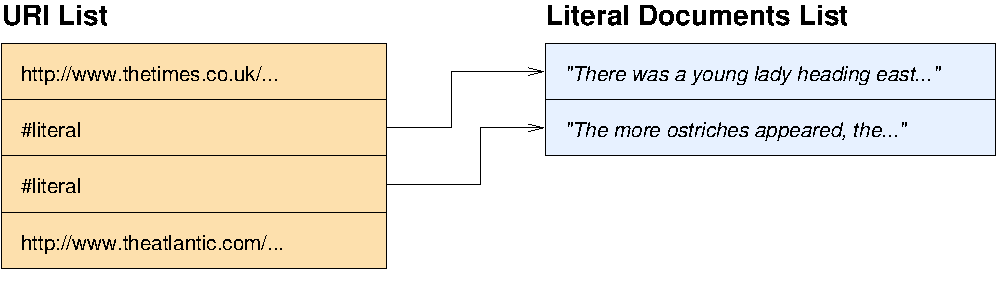
\includegraphics[width=0.8\textwidth]{pictures/twolists}
  \vspace*{-0.4cm}
  \caption{The two lists representing the input documents for an NLP service}  
  \label{fig:twolists}
\end{figure}

Besides the name and the input for a language service, we might need
the client to provide a list of parameters. Therefore, a list of
parameters as described in the previous section is passed along. The
\emph{Value} field of a parameter holds the user-specified value this
parameter should be assigned. Finally, we enable the communication of
user context by passing a representation thereof, as introduced in the
previous section. Table~\ref{tab:invocation} lists all the data
elements transmitted on language service invocation.

\begin{table}
 \centering\small\sffamily
 \begin{tabular}{p{0.22\textwidth}@{\hspace*{4mm}}p{0.45\textwidth}@{\hspace*{4mm}}p{0.2\textwidth}}
   \toprule
   \textbf{Field} & \textbf{Meaning} & \textbf{Example} \\
   \midrule
   NLP service name & The unique identifier of the desired & \emph{English Single} \\
    & language service & \emph{Document Summarizer} \\

    & & \\

   URI list & A list of actual input document URIs and special URIs
   signalling that this document is passed literally. Every input
   document is represented here. & See Fig.~\ref{fig:twolists}  \\

    & & \\

   Document text list & List of document texts, only of those
   documents that are passed literally & See Fig.~\ref{fig:twolists}
   \\

    & & \\

   Parameter list & Transports the parameter values that the client
   specifies & See Table~\ref{tab:param} \\

    & & \\

   User context & The user context, as specified in &
   \emph{[userLangs=en,fr} \\
    & Section~\ref{sec:contextservice} & \emph{docLang=en]}\\
 
   \bottomrule
\end{tabular}
 \caption{Data fields sent from the client when invoking an NLP service}
 \label{tab:invocation}
\end{table}

While language services can most likely be invoked without the current
user context at hand, knowing some facts can prove useful before or
after the invocation. Thus, the invocation could be cancelled if it
is detected that the chosen language service does not fit the input
document(s), or one could tailor the generated output to the user
client's preferences or capabilities.


\subsection{Language Service Results}
\label{sec:response}
Once a language service has finished its work, we want to collect its
results and pass them, in an appropriate format, on to the client. The
\sa architecture allows for different result formats (document
annotation, new documents, results files such as ontologies) and
passes them in a uniform XML response format back to the client.

The basic structure of our response message is rather simple. No
matter what the contents of a message are, they are always be enclosed
in a single \texttt{saResponse} element, the ``sa'' standing for
``Semantic Assistant''. Within this enclosing element, the results
produced by the language service are listed one by one. In
Figure~\ref{list:response1}, this is illustrated for a language
service which produces two different results. Here, they are called
\emph{result1} and \emph{result2}. In reality, they might be an
annotation and a file, or two different annotations, etc.

\begin{figure}[htb]
\begin{lstlisting}[language=XML,xleftmargin=8mm,columns=flexible]
<?xml version="1.0"?>
<saResponse>
    <result1>
        ...
    </result1>
    <result2>
        ...
    </result2>
</saResponse>
\end{lstlisting}
\caption{Schematic structure of an example response with two results}
\label{list:response1}
\end{figure}


\paragraph{GATE Annotations.} With the outer structure of a response
message in place, we have to properly define how specific results are
represented. We take care of annotations first, especially annotations
in GATE (see the GATE documentation for a description of the GATE
document data model if you do not know about document annotations).
Instead of \texttt{result1} or \texttt{result2} in the example above,
we will thus have \texttt{annotation} tags. An important aspect of an
annotation obviously is its name, or type, e.g., \emph{Protein} or
\emph{Person}.  Additionally, for GATE annotations, we include the
annotation set that the annotation is contained in. Thus, we have an
\texttt{annotation} element with \texttt{type} and
\texttt{annotationSet} attributes.

There might be several input document to an NLP service, and an
annotation is always associated with a specific document. Therefore, the
response first lists all input documents within each
\texttt{annotation} tag, using \texttt{document} tags. If the URL of a
document is known, it is included in the corresponding \texttt{document}
tag. However, if a document has been passed literally, we do not have
a URL, so we cannot include it in the response message either. This
seems to be a problem when several documents are passed literally: How
does the client know which result belongs to which document? However,
the order of the documents is maintained as it was when the client
sent them as input.  Therefore, the client is able to correctly assign
the results to the input documents.

For every document, we then list the occurrences of the annotation in
question, using \texttt{annotationInstance} elements. Instances hold a
\texttt{start} and an \texttt{end} attribute, which are character
offsets and which enable the client to locate the instance in the
input text. Moreover, there is a \texttt{content} attribute, which
holds the text located between the \texttt{start} and \texttt{end}
text positions. Finally, annotations can hold an arbitrary number of
so-called features. Features that the system integrator thinks could
be of interest are listed as child elements of the
\texttt{annotationInstance} elements. We can see an example output
with three different annotations (\emph{Date}, \emph{Person}, and
\emph{Location}) and one document in Figure~\ref{list:response2}. The
\emph{Person} and \emph{Location} annotations each have one feature
listed -- \emph{gender} in the case of the person, \emph{locType} in
the case of the location. The document has been passed via URL, which
is why this URL is also included in the response.

\begin{figure}[htb]
\begin{lstlisting}[language=XML,xleftmargin=8mm,columns=flexible]
<?xml version="1.0"?>
<saResponse>
  <annotation type="Date" annotationSet="">
    <document url="http://www.thetimes.co.uk/...">
      <annotationInstance content="yesterday" start="76" end="85">
      </annotationInstance>
      <annotationInstance content="today" start="1056" end="1061">
      </annotationInstance>
      <annotationInstance content="past ten years" start="6477" end="6491">
      </annotationInstance>
    </document>
  </annotation>
  <annotation type="Person" annotationSet="">
    <document url="http://www.thetimes.co.uk/...">
      <annotationInstance content="Tony Blair" start="65"  end="75">
        <feature name="gender" value="male" />
      </annotationInstance>
      <annotationInstance content="Rupert Murdoch" start="2357" end="2371">
        <feature name="gender" value="male" />
      </annotationInstance>
      <annotationInstance content="Mr Blair" start="3133"  end="3141">
        <feature name="gender" value="male" />
      </annotationInstance>
    </document>
  </annotation>
  <annotation type="Location"  annotationSet=""  >
    <document url="http://www.thetimes.co.uk/...">
      <annotationInstance content="Iraq" start="1510" end="1514">
        <feature name="locType" value="country" />
      </annotationInstance>
      <annotationInstance content="Downing Street" start="4576" end="4590">
        <feature name="locType" value="" />
      </annotationInstance>
    </document>
  </annotation>
</saResponse>
\end{lstlisting}
\vspace*{-2mm}
\caption{Result example with three annotations and their detected instances}
\label{list:response2}
\end{figure}

\paragraph{GATE Boundless Annotations.} Boundless annotations are special kind of annotations that adhere to the whole document and have no start and end offsets. Like Annotation instances, they may hold a list of features. The handling behaviour of such annotations depends on the invoking client's implementation.  

\paragraph{Result Files.} NLP services can also generate new files as
a result -- these can be of any format, depending on the concrete
components deployed in the pipeline. Instead of embedding the file
itself (which can be quite large) directly into the response, we only
pass an identifier for the file, along with some format information.
The client can evaluate this information, and, if it decides to do so,
request the result file itself by using the identifier sent to it. The
server then sends the actual file. Again, we have an example response
in Figure~\ref{list:response3}. The \texttt{outputFile} element holds
format information, both in form of a MIME type string and a human
readable one. This MIME type can be used by clients to decide the best suitable
presentation method. The identifier for the result file is given through the
\texttt{url} attribute which refers to the server's file system.

\begin{figure}
\begin{lstlisting}[language=XML,xleftmargin=8mm,columns=flexible]
<?xml version="1.0"?>
<saResponse>
  <outputFile url="file:/tmp/serviceResult-..."
              mimeType="text/html" format="HTML Document" />
</saResponse>
\end{lstlisting}
\vspace*{-2mm}
\caption{Result example with one resulting HTML file}
\label{list:response3}
\end{figure}


\paragraph{Formal Response Message Format Definition.} The complete
response format definition DTD can be found in
Figure~\ref{list:dtd}. It defines documents of the type
\texttt{saResponse}. The \texttt{saResponse} element can contain
arbitrarily many \texttt{annotation} elements and \texttt{outputFile}
elements. Annotations, annotation instances, features, and output
files are defined accordingly.

\begin{figure}
\begin{lstlisting}[language=XML,xleftmargin=8mm,columns=flexible]
<!DOCTYPE saResponse [

  <!ELEMENT saResponse ( annotation*, outputFile* ) >

  <!ELEMENT annotation ( document+ ) >
  <!ATTLIST annotation annotationSet CDATA #IMPLIED >
  <!ATTLIST annotation type NMTOKENS #REQUIRED >

  <!ELEMENT annotationInstance ( feature* ) >
  <!ATTLIST annotationInstance content CDATA   #REQUIRED >
  <!ATTLIST annotationInstance end     NMTOKEN #REQUIRED >
  <!ATTLIST annotationInstance start   NMTOKEN #REQUIRED >

  <!ELEMENT document ( annotationInstance* ) >
  <!ATTLIST document url CDATA #IMPLIED >

  <!ELEMENT feature EMPTY >
  <!ATTLIST feature name  NMTOKEN #REQUIRED >
  <!ATTLIST feature value CDATA   #REQUIRED >

  <!ELEMENT outputFile EMPTY >
  <!ATTLIST outputFile format   CDATA #REQUIRED >
  <!ATTLIST outputFile mimeType CDATA #REQUIRED >
  <!ATTLIST outputFile url      CDATA #REQUIRED >

]>
\end{lstlisting}
\vspace*{-2mm}
\caption{The document type definition (DTD) for our response messages}
\label{list:dtd}
\end{figure}

We have now discussed the most important data exchange processes. In
the next section, we want to ask the question where this data on NLP
services comes from, and how it is organized.

\section{Developing a New Client for the Semantic Assistants Architecture}
We have now covered the most important and interesting implementation
issues, and are ready, with the knowledge we have, to give
step-by-step instructions to connect a client application to our
architecture, and thus to the functionality of NLP services. These
instructions depend a bit on the client implementation language. As we
described earlier, our implementation of the client-side abstraction
layer consists of Java classes packaged in a single Java archive
(\texttt{.jar}) file. Hence, if the client application is able to make
use of Java archives, connecting to our architecture is done as
follows:

\begin{enumerate}
\item Have your application import the Java archive containing the
    implementation of the client-side abstraction layer (CSAL).

\item If necessary, tell the CSAL the address of the Web service
    endpoint. The CSAL classes that need to know the address have a
    default value for it.

\item Create a \texttt{SemanticServiceBrokerService} object, which
    serves as a factory for proxy objects.

\item Create such a proxy object. This is your ``remote control'' to
    the Web service. You can call all methods that have been published
    through the Web service on this object.
\end{enumerate}

After these four steps, a Java-enabled client application can get
lists of available language services as well as invoke these language
services. A code example, where an application obtains such a proxy
object and invokes the \texttt{getAvailableServices} method on it to
find available language analysis services, is shown below:

\begin{lstlisting}[language=Java,xleftmargin=4mm,columns=flexible]
// Create a factory object
SemanticServiceBrokerService service = new SemanticServiceBrokerService();
// Get a proxy object, which locally represents the service endpoint (= port)
SemanticServiceBroker broker = service.getSemanticServiceBrokerPort();
// Proxy object is ready to use. Get a list of available language services.
ServiceInfoForClientArray sia = broker.getAvailableServices();
\end{lstlisting}

A client application developer who cannot use the Java archive that
implements the CSAL still has access to the WSDL description of our
Web services. If there are automatic client code generation tools
available for the programming language of his choice, the developer
can use these to create CSAL-like code, which can then be integrated
into or imported by his application. In this case, the integration
steps would be similar to the steps enumerated above, with the
additional step of generating client-side code from the WSDL
description before the first step.

If there are no such code generation tools, the client application has
to implement the communication with the server itself. To do this, it
must create the SOAP messages that represent method invocations, and
send them to the Web service endpoint. Also, it must receive the
response messages from the server, and extract the relevant
information in them. Usually, however, there are standard libraries
that facilitate these tasks.

\subsection{Reusing CSAL Utility Classes}
The CSAL contains Java classes that define a set of methods that perform common, often re-used functions for clients to facilitate the interaction with the sever and consuming the results afterwards. It is encouraged that all the clients use these utility classes to ensure a unique presence and behavior among all the plug-ins.

\paragraph{Runtime Parameters Prompt Dialog.} There exists NLP pipelines that require mandatory runtime parameters which has to be acquired from the user prior to execution. This requirement has been fulfilled through a runtime parameter prompt dialog that pops up everytime the user invokes such an NLP pipeline. Since this dialog is used by all of the plug-ins, the prompt dialog - implemented as a swing dialog - has been placed in the CSAL in \texttt{RTParamFrame.java} class.

To use this dialog, import the RTParamFrame class into your program, provided that CSAL.jar file is on your project build path.

\begin{lstlisting}[language=Java,xleftmargin=4mm,columns=flexible]
import info.semanticsoftware.semassist.csal.RTParamFrame;
\end{lstlisting}

First of all, create an object of this class by passing the NLP service information as the input argument.  

\begin{lstlisting}[language=Java,xleftmargin=4mm,columns=flexible]
// The NLP service of choice
ServiceInfoForClient info = getAvailableServices().get( serviceName );

// Check whether this service actually requires mandatory runtime parameters
...

// If yes, create a new prompt dialog for the NLP service described in the 'info' argument
RTParamFrame frame = new RTParamFrame( info );   
\end{lstlisting}

Then you should extract the parameters to be shown in the dialog,
\begin{lstlisting}[language=Java,xleftmargin=4mm,columns=flexible]
Vector<GateRuntimeParameter> mandatory = new Vector<GateRuntimeParameter>();
Vector<GateRuntimeParameter> optional = new Vector<GateRuntimeParameter>();

// Read the mandatory and optional runtime parameters by investigating the 'info' parameters list
...

// Set the parameters
frame.setMandatories( mandatory );
frame.setOptionals( optional );
\end{lstlisting}

Next, you should override the frame's OK button ActionListener method and implement your own desired action.

\begin{lstlisting}[language=Java,xleftmargin=4mm,columns=flexible]
frame.setOkActionListener( new ParamActionListener() {
  ...
});
\end{lstlisting}

Finally, make it visible to the user.

\begin{lstlisting}[language=Java,xleftmargin=4mm,columns=flexible]
  frame.pack();
  frame.setVisible( true );
\end{lstlisting}

% \subsection{Control Flow Overview}
% \begin{figure}[htb]
%   \centering
%   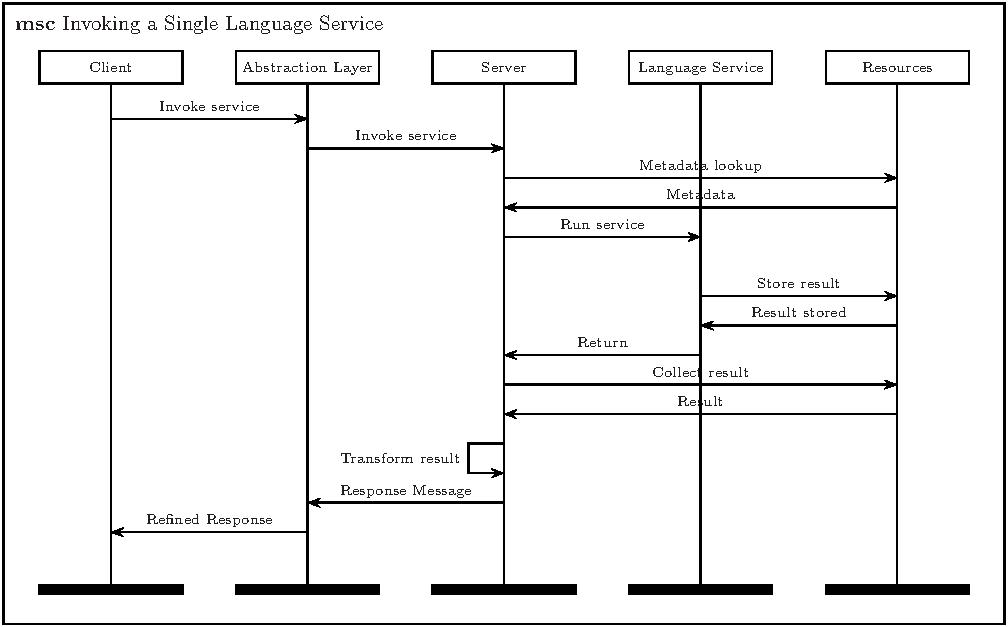
\includegraphics[width=0.5\textwidth]{pictures/seqInvoke1.pdf}
%   \caption{The client invokes a language service and receives a
%     result}
%   \label{fig:seqInvoke1}
% \end{figure}
% Once requested, the language service is executed asynchronously by our
% architecture, allowing the user to continue his work (he can even
% execute additional services).  The sequence diagram in
% Figure~\ref{fig:seqInvoke1} shows the execution of a service
% through the various tiers described in Section~\ref{sec:implementation} Note
% that all low-level details of handling language services, such as
% metadata lookup, parametrization, and result handling, are hidden from
% the client plug-in through our client-side abstraction layer.

\paragraph{Client Preference Management}
\label{client_pref}
As described in \ref{sec:pref_management}, the preference settings of Semantic Assistants clients are stored in a single shared XML file. Figure \ref{list:semassist-settings} presents the default structure of preference file. Initially, the settings file has a \texttt{<global>} tag. As the name suggests, all preferences stored as the children of this node will affect all the clients. The global tag has two \texttt{<server>} and one \texttt{<lastCalledServer>} child nodes that hold pre-defined server information for clients to connect to.
 
\begin{figure}[!tb]
\begin{lstlisting}[language=XML,xleftmargin=4mm,columns=flexible]
<?xml version="1.0" encoding="UTF-8" standalone="no"?>
<saProperties>
  <global>
    <lastCalledServer host="minion.cs.concordia.ca" port="8879"/>
    <server host="minion.cs.concordia.ca" port="8879"/>
    <server host="example.com" port="1234"/>
  </global>
</saProperties>
\end{lstlisting}
\caption{The \emph{semassist-settings.xml} file default structure}
\label{list:semassist-settings}
\end{figure}

Each client can store its proprietary preferences inside an XML tag that bears the client's name. For example, Figure \ref{list:eclipse-pref} shows the Eclipse plug-in preferred server information. The \texttt{ClientUtils.java} class inside CSAL.jar library provides methods to create and modify the preferences file. For more information on how to use the methods, please refer to the Javadoc documentation.

\begin{figure}[!tb]
\begin{lstlisting}[language=XML,xleftmargin=4mm,columns=flexible]
<eclipse>
  <server host="example.com" port="1234"/>
</eclipse>
\end{lstlisting}
\caption{The Eclipse plug-in preferences}
\label{list:eclipse-pref}
\end{figure}